\documentclass{beamer}
\usepackage{graphicx}
\usepackage{amssymb}
\usepackage{perpage}
\usepackage{beamerthemeshadow}

\mode<presentation>
{
  \usetheme{Frankfurt}
}

\setbeamertemplate{footline}[page number]
\usepackage[english]{babel}
\setbeamertemplate{navigation symbols}{}%remove navigation symbols
\newcommand{\bibintext}[1]{{\tiny \bibentry{#1}}}

\usepackage{bibentry}

\def\newblock{\hskip .11em plus .33em minus .07em}
\usepackage{times}

\title[elastic instabilities]{Smoothed dissipative particle dynamics simulations of elastic instabilities in diluted polymer solutions}
\date{}
\nobibliography*

\DeclareGraphicsRule{*}{mps}{*}{}

\author{S. Litvinov, X. Qingguang, M. Ellero, X.Y. Hu and N.A. Adams}

\institute{
  Lehrstuhl f\"{u}r Aerodynamik und Str\"{o}mungsmechanik \\
  TU M\"{u}nchen
}

\newcommand{\imgwidth}{0.92\textwidth}
\MakePerPage{footnote} %the perpage package command

\begin{document}
\begin{frame}
  \titlepage
\end{frame}

\begin{frame}
  \tableofcontents
\end{frame}

\section[Motivation]{Motivation}
\begin{frame}
  \frametitle{Motivation}
  \begin{columns}
    \begin{column}{0.5\textwidth}
      \begin{block}{Why polymer solutions?}
        \begin{itemize}
        \item Turbulent drag reduction
        \item Elastic instabilities and elastic turbulence leads to efficient mixing in microchannel flow
        \end{itemize}
      \end{block}
      \begin{block}{Why SDPD?}
        \begin{itemize} 
        \item Direct presentation of conformation of polymer molecules
        \item Easy measurement of elastic stress field
        \end{itemize}
      \end{block}

    \end{column}
    \begin{column}{0.5\textwidth}
\begin{figure}[t]
    \centering
    \includegraphics[width=0.6\textwidth]{img/polymers.png}
    \caption{Snapshot of polymer solutions in 2D.}
    \label{fig:snap}
  \end{figure}
    \end{column}
  \end{columns}
%   \footnotetext{\tiny \bibentry{baldassari2012flow}}
\end{frame}

\begin{frame}
  \frametitle{Motivation II}

  \begin{block}{Why Four-Roll Mill Flow?}
    \begin{itemize}
    \item Extensional flow is more effective to locally 
          stretch polymer molecules than simple shear flow
\item Polymer molecules are strongly stretched at extensional points in a micro-channel cross flow
    \end{itemize}

  \end{block}
The four-roll mill flow is driven by a steady background force in 2D:
\begin{equation}
\mathbf{F}=\left\{\begin{matrix}
C_0sin(\frac{2\pi x} {L})cos(\frac{2\pi x} {L})
\\ 
-C_0cos(\frac{2\pi x} {L})sin(\frac{2\pi x} {L})
\end{matrix}\right.
\end{equation}
%   \begin{block}{Viscosity}
%     $1<\text{Re}<2000$ $\implies$ full Navier-Stokes (NS) equations~\footnotemark
%   \end{block}
%   \footnotetext{\tiny \bibentry{worner_numerical_2012}}
\end{frame}

\begin{frame}
  \frametitle{Related Work}
\begin{block}{Numerical Simulation by Thomases et al. with DNS~\footnotemark: }
\begin{itemize}
 \item Beyond a first critical Wi number, the flow near the stagnation point becomes asymmetric and stretched.
\item At higher Wi number, the flow is dominated by a single large vortex and persistent oscillations occur. 
\end{itemize}
\end{block}
\begin{block}{Experiments by Liu et al.~\footnotemark[2]:}
\begin{itemize}
 \item  At low Wi the flow pattern is nearly Newtonian. 
\item At higher Wi, the strength and the position of the vortices fluctuates periodically.
\item At even higher Wi, the flow field fluctuates stochastically in space and time.
\end{itemize}
\end{block}
\footnotetext{\tiny \bibentry{Thomases2011}}
\footnotetext[2]{\tiny \bibentry{Liu2012}}
\end{frame}

% \begin{frame}
%   \frametitle{Models}
%   \begin{itemize}
%   \item VOF \\
%     \bibintext{welch_local_1995}, \\
%     \bibintext{kunkelmann_cfd_2009}
%   \item Lattice Boltzmann \\
%     \bibintext{markus_pool_2012}
%   \item Particle-Based \\
%     \bibintext{muller_particle-based_2005}, \\ 
%    \bibintext{yoon_direct_2001}
%   \end{itemize}
% \end{frame}

%%% Local Variables: 
%%% mode: latex
%%% TeX-master: t
%%% End: 

\section[Model]{Model}
% \begin{frame}
%   \frametitle{SDPD}
%    \begin{block}{}
%    SDPD is an extension of SPH method for mesoscopic scale by introducing thermal fluctuations in a consistent
% way through the fluctuation-dissipation theorem.
%   \end{block}
%  \begin{itemize}
%   \item \alert{SPH for Navier-Stokes Equation}
%   \item \alert{Thermal fluctuations} %~\footnotemark
%   \item \alert{Mechanical Modeling of the Polymer Molecule}%~\footnotemark[2]
%   \end{itemize}
% \end{frame}
% \begin{frame}
%   \frametitle{SPH for Navier-Stokes Equation}
% Navier-Stokes Equation
% \begin{equation}\label{equ:masscon}
%  \frac{d\rho}{dt}=-\rho\nabla\cdot\mathbf{v},
% \end{equation}
% \begin{equation}\label{equ:momecon}
%  \frac{\mathbf{dv}}{dt}=\mathbf{g}-\frac{1}{\rho}\mathbf{\nabla}p+\mathbf{F}
% \end{equation}

% SPH formulation:
%   \begin{equation}\label{equ:rho}
%  \rho_i=m_i \sum_j W_{ij}
% \end{equation}
%   \begin{equation}\label{equ:momeevo}
%  \frac{d\mathbf{v}_{i}^{(p)}}{dt}=-\frac{1}{m_i}\sum_j\left(\frac{p_i}{d_{i}^{2}}+\frac{p_j}{d_{j}^{2}}\right)\frac{\partial W}{\partial r_{ij}}\mathbf{e}_{ij},
% \end{equation}
% \begin{equation}\label{equ:acceleration}
%  \frac{d\mathbf{v}{_i}^{(v)}}{dt}=-\frac{\eta}{m_i}\sum_j\left(\frac{p^i}{d_{i}^{2}}+\frac{p^j}{d_{j}^{2}}\right)\frac{1}{r_{ij}}\frac{\partial W}{\partial r_{ij}}(\mathbf{e}_{ij}\cdot\mathbf{v}_{ij}\mathbf{e}_{ij}+\mathbf{v}_{ij}),
% \end{equation}
% \end{frame}

\begin{frame}[label=general]
  \frametitle{Simulation of Polymer in SDPD framework}
   \begin{columns}
    \begin{column}{0.6\textwidth}
      \begin{itemize}
      \item The  model of a polymer is a chain of SPH particles 
      \item Thermal fluctuations are taken into account according 
        to GENERIC in thermodynamically consistent way
      \item Bounded beads in addition to hydrodynamic interaction are
        subject to \textit{spring force}
      \end{itemize}      
    \end{column}    
    \begin{column}{0.5\textwidth}
      \begin{figure}
        \centering
        \includegraphics<1>[width=0.85\textwidth]{img/fin.png}
        \includegraphics<2>[width=0.85\textwidth]{img/vmdscene.png}
        \caption{Typical simulation configuration for 3D}
        \label{fig:fds}
      \end{figure}
    \end{column}    
  \end{columns}
\end{frame}

% \begin{frame}
%   \frametitle{Thermal fluctuations}
% % The irreversible part of the particle dynamic~\cite{Hu06} in SPH method is
% % \begin{eqnarray}\label{equ:thermal}
% % & &\dot{m}_i\vert_{irr}=0 \nonumber \\
% % & &\dot{\mathbf{P}}_i\vert_{irr}=\eta\sum_j\left(\frac{1}{d_{i}^{2}}+\frac{1}{d_{j}^{2}}\right)\frac{1}{r_{ij}}\frac{\partial W}{\partial r_{ij}}(\mathbf{e}_{ij}\cdot\mathbf{v}_{ij}\mathbf{e}_{ij}+\mathbf{v}_{ij})
% % \end{eqnarray}
% % According to the GENERIC formalism~\cite{Grmela1997}, thermal fluctuations can be take into account by postulating the mass and the momentum fluctuations
% % of particle $i$
% % \begin{eqnarray}\label{equ:thermalb}
% % & & d\tilde{m}_i=0 \nonumber \\
% % & & d\tilde{\mathbf{P}}_i=\sum_j B_{ij}d\bar{\mathscr{W}}_{ij}\cdot\mathbf{e}_{ij}
% % \end{eqnarray}
% % where $d\bar{\mathscr{W}}_{ij}$ is the traceless symmetric part of a matrix of independent increments of a Wiener process
% % $d\mathscr{W}_{ij}=d\mathscr{W}_{ji}$ i.e., $d\bar{\mathscr{W}}_{ij}=(d\mathscr{W}_{ij}+d\mathscr{W}_{ji}^T)/2-tr[d\mathscr{W}_{ij}]\mathbf{I}/D$.
% % \end{frame}
% % \begin{frame}
% The isothermal deterministic irreversible equations are:
% \begin{eqnarray}\label{equ:thermalfur}
%   & &\dot{m}_i\vert_{irr}=0  \nonumber \\
% & &\dot{\mathbf{P}}_i\vert_{irr}=-\sum_j\frac{B_{ij}^2}{4k_BT}
% (\mathbf{e}_{ij}\cdot\mathbf{v}_{ij}\mathbf{e}_{ij}+\mathbf{v}_{ij}),
% \end{eqnarray}
% where $k_B$ is the Boltzmann constant and $T$ is the system temperature, and $B_{ij}$ is
% \begin{equation}\label{equ:b}
%  B_{ij}=[-4k_BT\eta\left(\frac{1}{d_{i}^{2}}+\frac{1}{d_{j}^{2}}\right)\frac{1}{r_{ij}}\frac{\partial W}{\partial r_{ij}}]^{1/2}.
% \end{equation}
% \end{frame}

\begin{frame}
  \frametitle{Mechanical Modeling of the Polymer Chain}
Finitely extensible nonlinear elastic(FENE) springs
\begin{equation}\label{equ:fene}
 \mathbf{F}^{FENE}(\mathbf{r}_{ij})=\frac{K\mathbf{r}_{ij}}{1-(r/R_0)^2}
\end{equation}

FENE-E springs
  \begin{equation}\label{equ:feneE}
 \mathbf{F}^{FENE-E}(\mathbf{r}_{ij})=\frac{K(\mathbf{r}_{ij}-\delta)}{1-[(r-\delta)/R_0]^2}
\end{equation}
where $\delta$ is given minimal distance between neighboring beads.
\end{frame}

\begin{frame}
\frametitle{Numerical Setup} 
\begin{block}{A square periodic domain}
 \begin{itemize}
  \item total number of particles: $512 \times 512 = 262144$.
  \item domain size: $ 0.0128\times 0.0128$.
  \item polymer chains: $8$ beads and $16$ beads.
 \end{itemize}
\begin{table}
\begin{center}
  \begin{tabular}{| c | c | c |  c| c | c | c | c | c |}
    \hline
    Parameter & $\Delta x$ & $\rho$ & c & $\eta$ & $K$ & $R_0$ & $\delta$ \\ 
    \hline
    Value & $2.5E-5$ & 1 & 10 & 0.003 & 0.01 & 4.0 & 1.0 \\ 
   \hline
  \end{tabular}
\end{center}
\caption {The value of parameters in simulation}
\label{tab:roll}
\end{table}
\end{block}
\end{frame}



%%% Local Variables: 
%%% mode: latex
%%% TeX-master: t
%%% End: 

\section{Results}
\begin{frame}
  \frametitle{Flow of Pure Solvent}
%   \begin{itemize}
%   \item Initial condition: ``seed'' vapor particles in the center of
%     the domain
%   \item Domain is periodic, edges of the domain $T=T_s +
%     \Delta T$
%   \item Theory predicts a self similar temperature profile $T =
%     T(r/R(t))$, where $r$~---~distance from the center, $R(t)$~---~radius of
%     the bubble
%   \end{itemize}

\begin{figure}
    \centering
    \includegraphics[width=0.5\textwidth]{img/polymer_loc-15.png}
    \includegraphics[width=0.5\textwidth]{img/polymer_loc-9.png}
    \caption{Vorticity field and velocity of one point $P_0=[5/8L,5/8L]$ in flow of pure solvent flow at $Re\approx 80$.}
    \label{fig:vor_sol}
  \end{figure}
\end{frame}

\begin{frame}
  \frametitle{Flow of Polymer Solution}
  \begin{figure}
    \centering
    \includegraphics[width=0.6\textwidth]{img/polymer_loc-10.png}
  \includegraphics[width=0.5\textwidth]{img/polymer_loc-6.png}
    \caption{Vorticity field and elastic stress trace in flow of polymer solution at $Wi\approx1$.}
    \label{fig:vor_pol1}
  \end{figure}
\end{frame}

\begin{frame}
  \frametitle{Flow of Polymer Solution}
\begin{figure}[ht]
\includegraphics[width=0.5\textwidth]{img/polymer_loc-12.png}
\includegraphics[width=0.5\textwidth]{img/polymer_loc-7.png}
\caption{Vorticity field and velocity of the point $P_0$ in flow of polymer solution at $Wi\approx5$.}
\label{fug:vor_pol5}
\end{figure}
\end{frame}
% \begin{frame}
%   \frametitle{Flow of Polymer Solution}
%   \begin{figure}[ht]
% \includegraphics[width=0.5\textwidth]{img/polymer_loc-13.png}
% \includegraphics[width=0.5\textwidth]{img/polymer_loc-5.png}
% \caption{Velocity and elastic stress trace in flow of polymer solution at $Wi\approx5$.}
% \label{fug:vel_pol5}
% \end{figure}
% \end{frame}
\begin{frame}
  \frametitle{Flow of Polymer Solution}
  \begin{figure}[ht]
    \centering
    \includegraphics[width=0.5\textwidth]{img/polymer_loc-14.png}
    \includegraphics[width=0.5\textwidth]{img/polymer_loc-8.png}
    \caption{Vorticity field and velocity of the point $P_0$ in flow of polymer solution at $Wi\approx10$.}
    \label{fig:vor_pol10}
  \end{figure}
\end{frame}

\begin{frame}
 \frametitle{Flow of Polymer Solution}
  \begin{figure}[t]
    \centering
    \includegraphics[width=0.5\textwidth]{img/polymer_loc-11.png}
 \includegraphics[width=0.5\textwidth]{img/polymer_loc-0.png}
    \caption{Vorticity field and energy spectrum ($E_k\sim k^{-3.8}$) in flow of polymer solution at $Wi\approx10$ with perturbation.}
    \label{fig:vor_per}
  \end{figure}
\bibliographystyle{elsart-num}
\nobibliography{bibdata}
\end{frame}

%%% Local Variables: 
%%% mode: latex
%%% TeX-master: t
%%% End: 

\section{Conclusions}
\begin{frame}
  \frametitle{Conclusions}
  \begin{itemize}
  \item Particle based model for evaporation is proposed
  \item Heat supply is a rate limiting step: superheated and subheated
    liquid
  \item Model is tested for bubble growth and bubble departure
  \end{itemize}
\end{frame}

%%% Local Variables: 
%%% mode: latex
%%% TeX-master: t
%%% End: 



\begin{frame}
  \frametitle{Evaporation model: particle creation}
  \begin{block}{Rule}
    If a vapor particle has $T>T_s$ and has a liquid particle as a
    neighbor we create a new vapor particle
  \end{block}
  \begin{itemize}
  \item mass is from a liquid particle ($m_{liquid} >> m_{vapor}$)
  \item energy goes to vapor particle
  \item mechanical momentum is distributed between ``new'' and ``old''
    vapor particles
  \end{itemize}
\end{frame}

\section{Validation}
\begin{frame}
  \frametitle{A bubble growth}
  \begin{itemize}
  \item Initial condition: ``seed'' vapor particles in the center of
    the domain
  \item Domain is periodic, edges of the domain $T=T_s +
    \Delta T$
  \item Theory predicts a self similar temperature profile $T =
    T(r/R(t))$, where $r$~---~distance from the center, $R(t)$~---~radius of
    the bubble
  \end{itemize}
\end{frame}

\begin{frame}
  \frametitle{A bubble growth}
  \begin{figure}
    \centering
    \includegraphics[width=0.65\textwidth]{img/polymer_loc-14.png}
    \caption{Temperature profile at different times vs normalized
      distance from the center of the domain}
    \label{fig:self}
  \end{figure}
\end{frame}

\begin{frame}
  \frametitle{A bubble growth}
  \begin{figure}[ht]
    \centering
    \includegraphics[width=0.5\textwidth]{img/polymer_loc.png}
    \caption{Radius of the bubble vs time. Theory: $R(t) \propto \sqrt{t}$}
    \label{fig:dep}
  \end{figure}
\end{frame}

\begin{frame}
  \frametitle{Departure of the bubble from the wall}
  \begin{itemize}
  \item Bottom and top: wall, rest of the boundaries are periodic
  \item Initial condition: the bottom wall temperature $T=T_s + \Delta T$
  \item Initial condition: the bulk temperature $T=T_s$
  \item ``Seed'' vapor particles at the center of the bottom wall
  \item Buoyancy vs surface tension
  \end{itemize}
\end{frame}

\begin{frame}
  \frametitle{Departure of the bubble from the wall}
  \begin{figure}[ht]
    \centering
    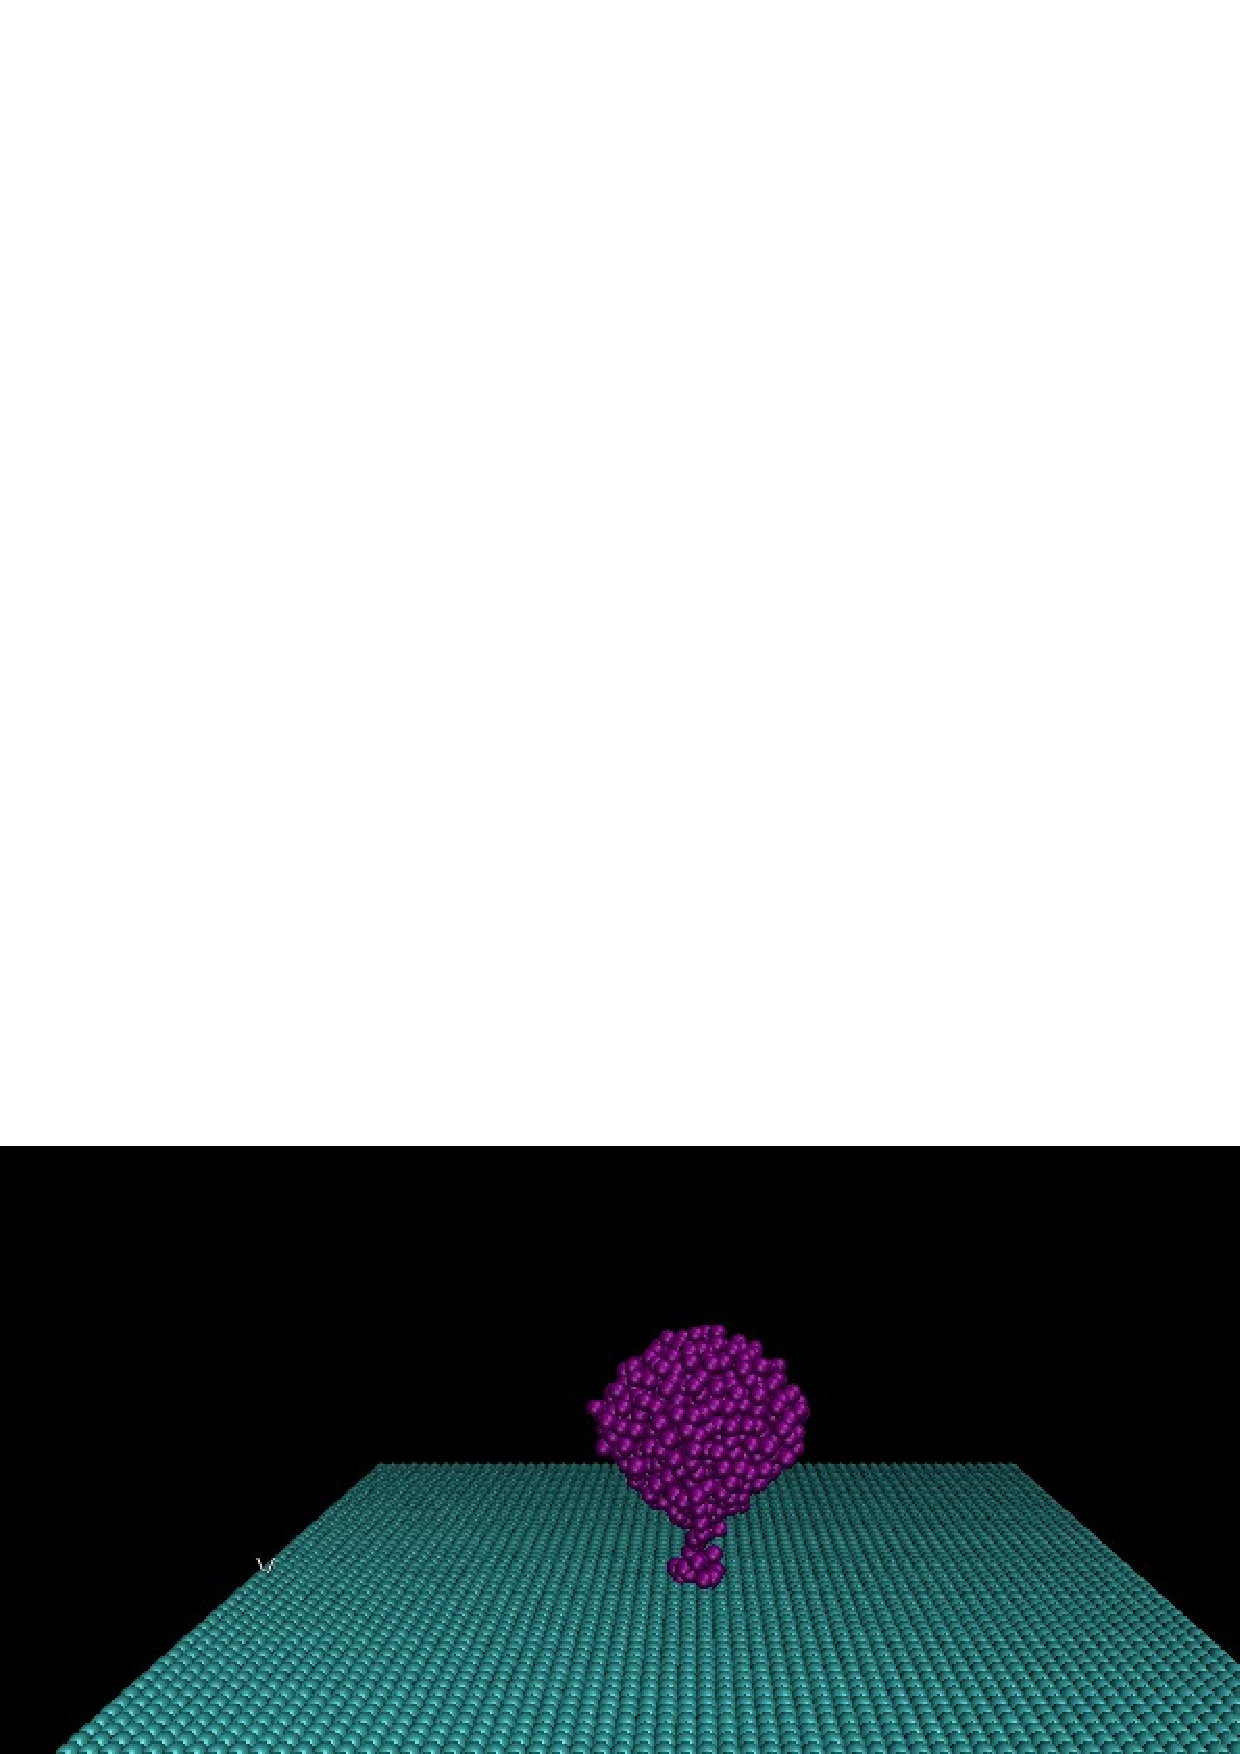
\includegraphics[width=0.8\textwidth]{gnuplot/dep-59.pdf}
    \caption{Snapshot of bubble departure from the super-heated
      surface. Liquid particles are not shown.}
    \label{fig:snapshot}
  \end{figure}
\end{frame}

\begin{frame}
  \begin{figure}[t]
    \centering
    \includegraphics{gnuplot/dep.pdf}
    \caption{Bubble departure radios versus gravity
      force. Theory:~$R_{dep} \propto 1/\sqrt{g})$ }
    \label{fig:radii}
  \end{figure}
  \bibliographystyle{elsart-num}
  \nobibliography{bibdata,intro}
\end{frame}

\section{Conclusions}
\begin{frame}
  \frametitle{Conclusions}
  \begin{itemize}
  \item Particle based model for evaporation is proposed
  \item Heat supply is a rate limiting step: superheated and subheated
    liquid
  \item Model is tested for bubble growth and bubble departure
  \end{itemize}
\end{frame}

\end{document}
